%%%%%%%%%%%%%%%%%%%%%%%%%%%%%%%%%%%%%%%%%%%%%%%%%%%%%
%			ŠABLONA PÍSNIČEK v. 18.09               %
%%%%%%%%%%%%%%%%%%%%%%%%%%%%%%%%%%%%%%%%%%%%%%%%%%%%%
% Tento soubor slouží jako (naučná) šablona, pomocí 
% které lze vytvářet zdrojové soubory k jednotlivým 
% písním.
%%%%%%%%%%%%%%%%%%%%%%%%%%%%%%%%%%%%%%%%%%%%%%%%%%%%%
%			Jak psát soubory songů?                 %
%%%%%%%%%%%%%%%%%%%%%%%%%%%%%%%%%%%%%%%%%%%%%%%%%%%%%
%	1. Text písně se začíná psát na místě START 
%	   a končí na místě END. Zbylý text ignorujte.
%	2. Jak bude vypadat pdf písně zjistíte po tom, 
%	   co soubor zkompilujete pomocí souboru   
%      ../Generator/generator. 
%	3. Při psaní dodržujte následující TeX pravidla:
%	 a) Nový řádek napíšete pomocí dvou odsazení 
%	    tedy dvou enterů.
%	 b) Nová sloka se píší pomocí \sloka a odsazení.
%		Refrén se píše jako \refren, v případě více 
%		refrénů \refren[č. refrénu].
%	 c) Akordy se píšou tak, že napíšete před slovo,
%	    kde chcete mít akord (bez mezery):
%		^{AKORD1\,AKORD2...}.
%	4. Pokud chcete ušetřit tvůrcům práci, tak 
%	   si přečtěte další poučný soubor o typografii 
%	   ../../Typo_pravidla.txt.
%	5. Akordy stačí psát jen do první sloky, když 
%	   se nezmění -- kytaristé to zvládnou
%	7. Název písně pište na místo [NÁZEV] a autora 
%	   pište na místo [AUTOR] 
%	7. Jak psát věci na české klávesnici:
%	   \ = alt gr + q; [/] = alt gr f/g; 
%      {/} = alt gr + b/n; ^ = alt gr + 3 , cokoliv
%%%%%%%%%%%%%%%%%%%%%%%%%%%%%%%%%%%%%%%%%%%%%%%%%%%%%
%			Jak kompilovat jednotlivé písně?        %
%%%%%%%%%%%%%%%%%%%%%%%%%%%%%%%%%%%%%%%%%%%%%%%%%%%%%
%	1. Více návodu je k tomuto napsáno v souboru 
%      ../Generator/generator. 
%%%%%%%%%%%%%%%%%%%%%%%%%%%%%%%%%%%%%%%%%%%%%%%%%%%%%
%			Jak kompilovat celý zpěvník?			%
%%%%%%%%%%%%%%%%%%%%%%%%%%%%%%%%%%%%%%%%%%%%%%%%%%%%%
%	1. Více návodu je k tomuto napsáno v souboru
%	   ../Cely_zpevnik/zpevnik.tex.
%%%%%%%%%%%%%%%%%%%%%%%%%%%%%%%%%%%%%%%%%%%%%%%%%%%%%
\begin{song}{title=\predtitle \centering Svaz českých bohémů \\\large Wohnout }  %% sem se napíše jméno songu a autor

\vspace*{.5cm}

\begin{centerjustified}
\vetsi

\predehra
\textbf{G Dmi Ami F C}

\refren
 ^{G\z}Vracím se domů nad ^{\z Dmi}ránem, kvalitním vínem ^{\z Ami}omámen,~~

   z přímek se stávaj ^*{\z F}zatáč ky, točí se ^{C\z}svět, jsem na ^{\z G}sračky.

   Vedle mě zvrací princezna, nastavím dlaň a požehnám, 

   pro všechny jasný poselství - tomu se říká přátelství. 


\sloka
Mám tisíc otázek na žádnou vzpomínku,

skládám si obrázek kámen po kamínku.

Včerejší produkce šla do bezvědomí,

nastává dedukce, co na to svědomí.

\sloka
A už si vzpomínám, já byl jsem na srazu,

s kumpány který mám, patříme do svazu,

vlastníme doménu, tak si nás rozklikni,

svaz českejch bohémů\elipsa.\elipsa.\elipsa.

\refren

\sloka
Stačí pár večírků, společně s bohémy,

za kterými se táhnou od školy problémy.

V partě je Blekota, Jekota, Mekota,

dost často hovoříme o smyslu života.

\sloka
Jako je třeba teď, mám tisíc otázek,

na žádnou vzpomínku, si skládám obrázek.

Z těžkejch ran lížu se, včera jsme slavili,

svatýho Vyšuse.

\refren

\end{centerjustified}
\newpage
\begin{centerjustified}

\sloka
Svět zrychluje svý otáčky,

sousedka peče koláčky.

Hlášen stav nouze nejvyšší,

Hapkové volaj Horáčky.

Zástupy českejch bohému,

vyráží ven do terénů

šavlí z kvalitního vína

bojovat proti systému.

\sloka
/: Tak jsme se tu všichni sešli, co myslíš, osobo?

Na to nelze říci než \uv{Co je ti do toho?}

Tak jsme se tu všichni sešli, co myslíš, osude?

Na to nelze říci než \uv{Jinak to nebude.}:/

Tak jsme se tu všichni sešli, co myslíš, osobo?

Na to nelze říci než \uv{Co je ti do toho?}

Tak jsme se tu všichni sešli, co myslíš, osude?

Na to nelze říci než \uv{Jinak to nebude.}

\vspace{1cm}

\ssloka{Pozn.} 
krom akordů doprovázejte:
\centering
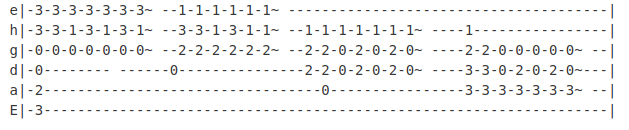
\includegraphics[scale=.75]{../taby/svazceskychbohemu.png}

\end{centerjustified}
\setcounter{Slokočet}{0}
\end{song}
